% Provenance (never printed): see sources/outline_sources.md (Year 1:
% geological cross-sections, apparent dip, thickness, boreholes). Every
% Varden Hills number comes from figdata/bachelor-1/varden_sections.py, which
% imports the shared model figdata/shared/region.py; numbers of the exercises
% and problem in the Book 3 scratch calculator and in that script's values.
\chapter{المقاطع الجيولوجية}\label{ch:b1:cross-sections}

تخطّط شركة هندسية نفقًا تحت تلال فاردن، مستقيمًا من الغرب إلى الشرق على ارتفاع ثابت قدره \qty{200}{m}. وقبل أن يُحفر متر واحد، يجب على الجيولوجيين أن يقولوا أيّ الصخور ستقطعها الآلة، وأين ستعبر الصدع، وكم ستقضي في الحجر الجيري، وهو صخر قد يحوي تجاويف مفتوحة ومياهًا. لا أحد يرى داخل التلال؛ لكن \omterm{def:b1:geological-maps:geological-map}{الخريطة الجيولوجية} في \cref{ch:b1:geological-maps}، وبعض الآبار الاستكشافية، وهندسة المستويات، تكفي لرسم شريحة شاقولية في الأرض ---
وهي \omterm{def:b1:cross-sections:section}{المقطع الجيولوجي} --- ولقراءة الأجوبة منها. يعلّم هذا الفصل كيف يُبنى المقطع انطلاقًا من الخريطة، وكيف تتغيّر الميول والسُّمك حين تُقطع الشريحة مائلةً، وكيف تُطابَق الآبار، وكيف يروي المقطع تاريخ الصخور التي يقطعها. ويختم بالنفق.

\begin{recall}
تُعطى \omterm{def:b1:geological-maps:attitude}{وضعية المستوي} بانحداره الاتجاهي $\alpha$ وانحداره $\delta$، والمستوي الذي يمرّ بنقطة ارتفاعها $z_0$ عند نقطة الأصل هو
$z = z_0 - \tan\delta\,(x\sin\alpha + y\cos\alpha)$؛ وثلاث نقاط من \omterm{def:b1:geological-maps:geological-map}{تماس} تحدّد وضعيته؛ وقاعدة V تقرأ \omterm{def:b1:geological-maps:attitude}{الانحدار} من نمط \omterm{def:b1:geological-maps:geological-map}{الانكشاف} في الوديان (\cref{ch:b1:geological-maps}). والكنتور يصل بين النقاط ذات الارتفاع المتساوي على الخريطة الطبوغرافية (الكتاب 1، الصف 9). والصخور الأحدث تقع فوق الأقدم، وكل ما يقطع صخرًا فهو أحدث منه (الكتاب 1، الصف 7).
\end{recall}

\section{من الخريطة إلى المقطع}

\begin{definition}[المقطع الجيولوجي، والمقطع الطبوغرافي، والمبالغة الرأسية]\label{def:b1:cross-sections:section}
\emph{المقطع الجيولوجي}\index{المقطع الجيولوجي} رسم للوحدات الصخرية والبنى في مستوٍ شاقولي يمرّ بالأرض، على خط مرسوم على الخريطة. وحافته العليا هي \emph{المقطع الطبوغرافي}\index{المقطع الطبوغرافي}، أي منحنى ارتفاع الأرض على طول الخط. و\emph{المبالغة الرأسية}\index{المبالغة الرأسية} $e$ للمقطع هي نسبة مقياسه الرأسي إلى مقياسه الأفقي؛ ويكون المقطع \emph{بالمقياس الحقيقي} عندما يكون $e = 1$.
\end{definition}

\begin{method}[بناء مقطع جيولوجي انطلاقًا من الخريطة]\label{met:b1:cross-sections:construct}
\begin{enumerate}
  \item ارسم خط المقطع على الخريطة، وضع حافة شريط من الورق عليه؛ علّم أين يعبر كل خط كنتور، مع ارتفاعه، وأين يعبره كل \omterm{def:b1:geological-maps:geological-map}{تماس} وكل صدع.
  \item ارسم خطًّا قاعديًّا أفقيًا بالطول نفسه ومقياسًا رأسيًا للارتفاع (اختر $e$، واكتبه على المقطع).
  \item انقل كل علامة كنتور إلى ارتفاعها، ووصل النقاط وصلًا ناعمًا: هذا هو \omterm{def:b1:cross-sections:section}{المقطع الطبوغرافي}.
  \item انقل كل \omterm{def:b1:geological-maps:geological-map}{تماس} وكل صدع إلى \omterm{def:b1:cross-sections:section}{المقطع الطبوغرافي}، عند النقطة التي يعبر عندها الخط.
  \item من كل نقطة من هذه، ارسم \omterm{def:b1:geological-maps:geological-map}{التماس} داخل الأرض بانحداره \emph{في مستوي المقطع} --- وهو \omterm{def:b1:cross-sections:apparent-dip}{الانحدار الظاهري} (\cref{sec:b1:cross-sections:apparent}) --- مضخّمًا بالعامل $e$ إذا كان $e \ne 1$؛ واستعمل الآبار والكنتورات البنيوية حيث توجد.
  \item أكمِل الوحدات بين \omterm{def:b1:geological-maps:geological-map}{التماسات}، مع احترام تتابع التراكب والقطع، وأضف المفتاح والمقاييس واتجاه الخط و$e$.
\end{enumerate}
\end{method}

\begin{omfigure}
\begin{tikzpicture}[font=\scriptsize, x=1cm, y=1cm]
% map strip with contours crossing the section line
\draw[black!50] (0,2.7) rectangle (9,4.5);
\foreach \x/\h in {0.7/300, 1.6/350, 2.6/400, 4.1/400, 5.0/350, 5.8/300, 7.2/300, 8.2/350} {
  \draw[contour, brown!70!black] (\x-0.25,2.7) .. controls (\x+0.1,3.4) and (\x-0.1,3.8) .. (\x+0.2,4.5);
  \node[brown!60!black, above] at (\x+0.2,4.5) {\h};
}
\draw[omThm, thick] (0,3.6) node[left] {X} -- (9,3.6) node[right] {Y};
\fill[omDef] (3.4,3.6) circle (1.5pt);
\node[omDef, fill=white, inner sep=1pt, above right] at (3.4,3.62) {تماس};
% profile
\draw[->] (0,-0.1) -- (0,1.95) node[above] {\foreignlanguage{arabic}{الارتفاع \babelsublr{(m)}}};
\draw (0,0) -- (9,0);
\foreach \y/\l in {0/250, 0.5/300, 1.0/350, 1.5/400} { \draw (-0.08,\y) -- (0,\y); \node[left] at (-0.08,\y) {\l}; }
\coordinate (p1) at (0.85,0.5); \coordinate (p2) at (1.75,1.0); \coordinate (p3) at (2.75,1.5);
\coordinate (p4) at (4.25,1.5); \coordinate (p5) at (5.15,1.0); \coordinate (p6) at (5.95,0.5);
\coordinate (p7) at (7.35,0.5); \coordinate (p8) at (8.35,1.0);
\foreach \i/\x in {1/0.85,2/1.75,3/2.75,4/4.25,5/5.15,6/5.95,7/7.35,8/8.35} {
  \draw[black!35, densely dotted] (\x,3.6) -- (p\i);
  \fill (p\i) circle (1.2pt);
}
\draw[thick] (0,0.2) .. controls (0.5,0.3) .. (p1) .. controls (1.3,0.8) .. (p2) .. controls (2.3,1.35) .. (p3)
  .. controls (3.5,1.85) .. (p4) .. controls (4.7,1.25) .. (p5) .. controls (5.5,0.7) .. (p6)
  .. controls (6.6,0.25) .. (p7) .. controls (7.9,0.75) .. (p8) .. controls (8.7,1.15) .. (9,1.2);
\draw[omDef, densely dotted] (3.4,3.6) -- (3.4,1.72);
\draw[omDef, thick] (3.4,1.72) -- (4.45,0.05);
\node[omDef, below right] at (4.3,-0.02) {تماس، مرسوم بانحداره الظاهري};
\end{tikzpicture}

{\small بناء مقطع (تخطيطي): تُنقل تقاطعات خطوط الكنتور مع الخط X--Y إلى ارتفاعاتها لتعطي \omterm{def:b1:cross-sections:section}{المقطع الطبوغرافي}؛ ويُنقل تماسٌ يعبر الخط إلى \omterm{def:b1:cross-sections:section}{المقطع الطبوغرافي}، ويُرسم داخل الأرض بانحداره الظاهري.}
\end{omfigure}

سيُبنى المقطع أدناه بالحاسوب من نموذج تلال فاردن على طول الخط C--D، الذي يمتد شرقًا مباشرةً عبر الخريطة عند $y = \qty{6}{km}$. ويُظهر \omterm{def:b1:geological-maps:fold}{الطية المحدبة} التي يظهر لبّها من الحجر الرملي والأساس عند $x \approx \qty{3.5}{km}$، والحجر الجيري والصخر الطيني على جناحيها، والطباشير في \omterm{def:b1:geological-maps:fold}{الطية المقعرة} إلى الشرق، والصدع العادي. ويُرسم عليه خط النفق عند \qty{200}{m}، والآبار الاستكشافية B1 وB2 وB3 الواردة في \cref{sec:b1:cross-sections:boreholes}.

\begin{omfigure}
\begin{tikzpicture}
\begin{axis}[x=1.4cm, y=0.0042cm, xmin=0, xmax=10, ymin=-500, ymax=650,
  axis on top, tick label style={font=\scriptsize}, label style={font=\small},
  xlabel={\foreignlanguage{arabic}{المسافة شرقًا من C \babelsublr{(km)}}}, ylabel={\foreignlanguage{arabic}{الارتفاع \babelsublr{(m)}}},
  ytick={-400,-200,0,200,400,600}, clip=true]
\addplot[lith schist, draw=black, line width=0.3pt, even odd rule] table {figdata/out/bachelor-1-varden_sections-cd-unit-schist.dat};
\addplot[lith granite, draw=black, line width=0.3pt, even odd rule] table {figdata/out/bachelor-1-varden_sections-cd-unit-granite.dat};
\addplot[om lith={icsTriassic!35}{om sand}, draw=black, line width=0.3pt, even odd rule] table {figdata/out/bachelor-1-varden_sections-cd-unit-sandstone.dat};
\addplot[om lith={icsJurassic!40}{om limestone}, draw=black, line width=0.3pt, even odd rule] table {figdata/out/bachelor-1-varden_sections-cd-unit-limestone.dat};
\addplot[om lith={icsJurassic!15}{om shale}, draw=black, line width=0.3pt, even odd rule] table {figdata/out/bachelor-1-varden_sections-cd-unit-shale.dat};
\addplot[om lith={icsCretaceous!35}{om limestone}, draw=black, line width=0.3pt, even odd rule] table {figdata/out/bachelor-1-varden_sections-cd-unit-chalk.dat};
\addplot[lith alluvium, draw=black, line width=0.3pt, even odd rule] table {figdata/out/bachelor-1-varden_sections-cd-unit-alluvium.dat};
\addplot[black, line width=0.8pt] table {figdata/out/bachelor-1-varden_sections-cd-ground.dat};
\addplot[fault, line width=1.1pt] table {figdata/out/bachelor-1-varden_sections-cd-fault.dat};
\addplot[omThm, line width=1.4pt] coordinates {(1,200) (9,200)};
\node[omThm, font=\scriptsize, fill=white, inner sep=1pt, below] at (axis cs:8.3,190) {النفق، \qty{200}{m}};
\draw[blue!60!black, line width=0.9pt] (axis cs:1.5,-480) -- (axis cs:1.5,524);
\draw[blue!60!black, line width=0.9pt] (axis cs:3.5,-480) -- (axis cs:3.5,381);
\draw[blue!60!black, line width=0.9pt] (axis cs:5.5,-480) -- (axis cs:5.5,530);
\node[font=\scriptsize, blue!60!black, fill=white, inner sep=1pt] at (axis cs:1.5,-440) {B1};
\node[font=\scriptsize, blue!60!black, fill=white, inner sep=1pt] at (axis cs:3.5,-440) {B2};
\node[font=\scriptsize, blue!60!black, fill=white, inner sep=1pt] at (axis cs:5.5,-440) {B3};
\node[font=\small, above right] at (axis cs:0,650) {\foreignlanguage{arabic}{C (غرب)}};
\node[font=\small, above left] at (axis cs:10,650) {\foreignlanguage{arabic}{D (شرق)}};
\end{axis}
\end{tikzpicture}

\smallskip
\begin{tikzpicture}
\begin{axis}[x=1.4cm, y=0.0014cm, xmin=0, xmax=10, ymin=-500, ymax=650,
  axis on top, tick label style={font=\scriptsize}, ytick={-500,0,500},
  xticklabels={}, clip=true]
\addplot[lith schist, draw=black, line width=0.2pt, even odd rule] table {figdata/out/bachelor-1-varden_sections-cd-unit-schist.dat};
\addplot[lith granite, draw=black, line width=0.2pt, even odd rule] table {figdata/out/bachelor-1-varden_sections-cd-unit-granite.dat};
\addplot[om lith={icsTriassic!35}{om sand}, draw=black, line width=0.2pt, even odd rule] table {figdata/out/bachelor-1-varden_sections-cd-unit-sandstone.dat};
\addplot[om lith={icsJurassic!40}{om limestone}, draw=black, line width=0.2pt, even odd rule] table {figdata/out/bachelor-1-varden_sections-cd-unit-limestone.dat};
\addplot[om lith={icsJurassic!15}{om shale}, draw=black, line width=0.2pt, even odd rule] table {figdata/out/bachelor-1-varden_sections-cd-unit-shale.dat};
\addplot[om lith={icsCretaceous!35}{om limestone}, draw=black, line width=0.2pt, even odd rule] table {figdata/out/bachelor-1-varden_sections-cd-unit-chalk.dat};
\addplot[lith alluvium, draw=black, line width=0.2pt, even odd rule] table {figdata/out/bachelor-1-varden_sections-cd-unit-alluvium.dat};
\addplot[black, line width=0.6pt] table {figdata/out/bachelor-1-varden_sections-cd-ground.dat};
\addplot[fault, line width=0.8pt] table {figdata/out/bachelor-1-varden_sections-cd-fault.dat};
\end{axis}
\end{tikzpicture}

{\small مقطع C--D عبر تلال فاردن، من نموذج المنطقة. أعلى: \omterm{def:b1:cross-sections:section}{المبالغة الرأسية} $e = 3$؛ وأسفل: المقطع نفسه بالمقياس الحقيقي ($e = 1$)، حيث تبدو الجناحان البالغ ميلهما \ang{12} لطيفين كما هما. الألوان كما في \omterm{def:b1:geological-maps:geological-map}{الخريطة الجيولوجية} في \cref{ch:b1:geological-maps}؛ والصدع (الخط السميك) هو الصدع العادي، وكتلته الشرقية هابطة. والخط الأحمر هو نفق المسألة؛ وB1--B3 آبار استكشافية.}
\end{omfigure}

\omterm{def:b1:cross-sections:section}{المبالغة الرأسية} تُظهر الوحدات الرقيقة والتضاريس اللطيفة بوضوح، لكنها تشوّه كل زاوية: إذ تظهر الجناحان البالغ ميلهما \ang{12} \omterm{def:b1:geological-maps:fold}{للطية} نحو \ang{32} تقريبًا في المقطع العلوي. والفرع التالي يبيّن ذلك بالدقة.

\section{الانحدار الظاهري}\label{sec:b1:cross-sections:apparent}

\begin{definition}[الانحدار الظاهري]\label{def:b1:cross-sections:apparent-dip}
\emph{الانحدار الظاهري}\index{الانحدار الظاهري} $\beta$ لمستوٍ في مقطع شاقولي معيّن هو الزاوية بين الأفق وأثر المستوي في ذلك المقطع. وهو يساوي \omterm{def:b1:geological-maps:attitude}{الانحدار} الحقيقي $\delta$ حين يمتد المقطع على طول \omterm{def:b1:geological-maps:attitude}{اتجاه الانحدار}، ويساوي الصفر حين يمتد على طول \omterm{def:b1:geological-maps:attitude}{الامتداد}.
\end{definition}

\begin{theorem}[الانحدار الظاهري]\label{thm:b1:cross-sections:apparent-dip}
مستوٍ انحداره $\delta$ واتجاه انحداره $\alpha$، يقطعه مقطع شاقولي سمته $\theta$، يُظهر \omterm{def:b1:cross-sections:apparent-dip}{الانحدار الظاهري} $\beta$ بحيث
\[
  \tan\beta = \tan\delta\,\cos\gamma, \qquad \gamma = \alpha - \theta ,
\]
ويهبط المستوي في الاتجاه $\theta$ حين يكون $\cos\gamma > 0$.
وعلى الخصوص $|\beta| \le \delta$، مع المساواة فقط على طول \omterm{def:b1:geological-maps:attitude}{اتجاه الانحدار}.
\end{theorem}

\begin{proof}
خذ المستوي $z = z_0 - \tan\delta\,(x\sin\alpha + y\cos\alpha)$ من
\cref{ch:b1:geological-maps}. على طول المقطع، خطوة أفقية طولها $s$ في الاتجاه $\theta$ هي $(x, y) = s(\sin\theta, \cos\theta)$، إذن
$z = z_0 - s\tan\delta\,(\sin\theta\sin\alpha + \cos\theta\cos\alpha) =
z_0 - s\tan\delta\cos(\alpha - \theta)$. والأثر خط مستقيم يهبط بمقدار $\tan\delta\cos\gamma$ لكل وحدة مسافة أفقية: وهذا هو
$\tan\beta$. وبما أن $|\cos\gamma| \le 1$، فإن $|\tan\beta| \le \tan\delta$.
\end{proof}

\begin{omfigure}
\begin{tikzpicture}[font=\scriptsize, x={(1cm,0cm)}, y={(0.6cm,0.45cm)}, z={(0cm,1cm)}]
% hidden edges of the block
\draw[black!30, densely dashed] (0,0,0) -- (0,3,0) -- (4,3,0);
\draw[black!30, densely dashed] (0,3,0) -- (0,3,2);
% the oblique vertical section, from the front-left corner to the back-right one
\fill[black!10, opacity=0.7] (0,0,0) -- (4,3,0) -- (4,3,2) -- (0,0,2) -- cycle;
\draw[black!45] (0,0,0) -- (4,3,0) -- (4,3,2);
% the dipping plane, from the top-west edge down to the base
\fill[omDef!25, opacity=0.75] (0,0,2) -- (2.6,0,0) -- (2.6,3,0) -- (0,3,2) -- cycle;
\draw[omDef] (2.6,0,0) -- (2.6,3,0);
\draw[omDef, very thick] (0,0,2) -- (2.6,0,0);
\draw[omThm, very thick] (0,0,2) -- (2.6,1.95,0);
% visible edges of the block
\draw[black!70] (0,0,0) -- (4,0,0) -- (4,0,2) -- (0,0,2) -- cycle;
\draw[black!70] (0,0,2) -- (0,3,2) -- (4,3,2) -- (4,0,2);
\draw[black!70] (4,0,0) -- (4,3,0) -- (4,3,2);
% labels
\draw[omDef] (2.0,0,0) arc[start angle=180, end angle=142.4, radius=0.6cm];
\node[omDef] at (1.7,0,0.2) {$\delta$};
  \node[omDef, below, align=center] at (1.3,0,0) {الوجه الأمامي، على طول اتجاه الانحدار:\\ الانحدار الحقيقي $\delta$};
  \node[omThm, right, align=left] at (4.45,2.2,0.3) {المقطع المائل (الرمادي):\\ الانحدار الظاهري $\beta < \delta$};
  \node[above] at (0,1.5,2) {ش};
\draw[->] (0.15,1.5,2.05) -- (0.15,2.2,2.05);
\end{tikzpicture}

{\small \omterm{def:b1:cross-sections:apparent-dip}{الانحدار الظاهري} (كتلة تخطيطية). مستوٍ ينحدر نحو الشرق (بالأزرق) يُظهر انحداره الحقيقي $\delta$ على الوجه الأمامي، وهو وجه شاقولي مقطوع على طول \omterm{def:b1:geological-maps:attitude}{اتجاه الانحدار}؛ وعلى المقطع الشاقولي الرمادي، المقطوع مائلًا، يهبط أثره (بالأحمر) بانحدار أقلّ لطفًا، هو \omterm{def:b1:cross-sections:apparent-dip}{الانحدار الظاهري} $\beta$؛ وعلى مقطع على طول \omterm{def:b1:geological-maps:attitude}{الامتداد}، أي شمالي جنوبي، سيكون أفقيًا.}
\end{omfigure}

\begin{proposition}[الزوايا في مقطع مبالغ فيه]\label{prop:b1:cross-sections:exaggeration}
في مقطع مرسوم \omterm{def:b1:cross-sections:section}{بالمبالغة الرأسية} $e$، يُرسم خط انحداره الظاهري $\beta$ بالزاوية $\beta'$ حيث $\tan\beta' = e\tan\beta$.
\end{proposition}

\begin{proof}
نقيس الهبوط على مسافة أفقية $s$: يهبط الخط بمقدار $s\tan\beta$؛ ومرسومًا بمقياس رأسي يساوي $e$ مرة المقياس الأفقي، يظهر الهبوط بمقدار $es\tan\beta$ على الطول المرسوم نفسه $s$.
\end{proof}

\begin{example}
الجناح الشرقي \omterm{def:b1:geological-maps:fold}{لطية} فاردن ينحدر بزاوية \ang{12.16} نحو \ang{080.7} (\cref{ch:b1:geological-maps}). وفي المقطع شرق-غرب C--D، يكون $\gamma = \ang{80.7} - \ang{90} = \ang{-9.3}$، و$\tan\beta =
\tan\ang{12.16}\cos\ang{9.3} = 0.2154\times0.9868 = 0.2126$: $\beta =
\ang{12.0}$. ومرسومًا بالمبالغة $e = 3$ يظهر بالزاوية $\arctan(3\times0.2126) =
\ang{32.5}$. وفي المقطع A--B ذي \omterm{def:b1:spherical-astronomy:horizontal}{السمت} \ang{071.6}، يكون $\gamma = \ang{9.1}$ و$\beta = \ang{12.0}$ أيضًا: فالمقطعان يمتدان قريبًا من \omterm{def:b1:geological-maps:attitude}{اتجاه الانحدار}. والصدع، الذي ينحدر بزاوية \ang{60} نحو \ang{120}، له في C--D \omterm{def:b1:cross-sections:apparent-dip}{الانحدار الظاهري} $\arctan(\tan\ang{60}\cos\ang{30}) = \arctan 1.5 = \ang{56.3}$.
\end{example}

\section{السُّمك}

\begin{definition}[السمك الحقيقي، والسمك الشاقولي]\label{def:b1:cross-sections:thickness}
\emph{السمك الحقيقي}\index{السمك الحقيقي} $t$ لطبقة هو المسافة بين قاعدتها وقمتها مقيسةً عموديًا على التطبّق. و\emph{السمك الشاقولي}\index{السمك الشاقولي} $h$ هو المسافة نفسها مقيسةً على الشاقول، كما يقطعها بئر شاقولي.
\end{definition}

\begin{proposition}[سُمك طبقة مائلة]\label{prop:b1:cross-sections:thickness}
من أجل طبقة انحدارها $\delta$:
\begin{enumerate}
  \item $t = h\cos\delta$؛
  \item على أرض أفقية، إذا كان عرض \omterm{def:b1:geological-maps:geological-map}{انكشاف} الطبقة $w$ مقيسًا عموديًا على \omterm{def:b1:geological-maps:attitude}{الامتداد}، فإن $t = w\sin\delta$؛
  \item على أرض تميل بالزاوية $\sigma$ في الاتجاه العمودي على \omterm{def:b1:geological-maps:attitude}{الامتداد}، مع قياس $w$ على طول الأرض، يكون $t = w\sin(\delta + \sigma)$ إذا كانت الأرض تميل عكس \omterm{def:b1:geological-maps:attitude}{اتجاه الانحدار}، و$t = w\sin(\delta - \sigma)$ إذا كانت تميل في الاتجاه نفسه بانحدار أقلّ من انحدار الطبقات.
\end{enumerate}
\end{proposition}

\begin{proof}
في المستوي الشاقولي العمودي على \omterm{def:b1:geological-maps:attitude}{الامتداد}، تكون قاعدة الطبقة وقمتها خطين متوازيين مائلين بالزاوية $\delta$، والمسافة بينهما $t$. (1) قطعة شاقولية تصل بينهما تصنع الزاوية $\delta$ مع ناظمهما المشترك، إذن $t = h\cos\delta$. (2)--(3) قطعة طولها $w$ تصل بينهما على الأرض تصنع مع التطبّق الزاوية $\delta$ حين تكون الأرض مستوية، و$\delta + \sigma$ حين ترتفع الأرض نحو عكس \omterm{def:b1:geological-maps:attitude}{اتجاه الانحدار} (فالميلان يتجمعان)، و$\delta - \sigma$ حين تنخفض في الاتجاه نفسه؛ والمسافة بين الخطين المتوازيين هي طول القطعة مضروبًا في جيب تلك الزاوية.
\end{proof}

\begin{omfigure}
\begin{tikzpicture}[font=\scriptsize]
\pgfmathsetmacro{\d}{25}\pgfmathsetmacro{\t}{1.3}
\pgfmathsetmacro{\h}{\t/cos(\d)}\pgfmathsetmacro{\w}{\t/sin(\d)}
\pgfmathsetmacro{\X}{4.0}
\fill[icsJurassic!30] (-\w,0) -- (0,0) -- (\X,{-\X*tan(\d)}) -- (\X,{-\X*tan(\d)-\h}) -- cycle;
\draw[thick] (0,0) -- (\X,{-\X*tan(\d)}) node[right] {قمة الطبقة};
\draw[thick] (-\w,0) -- (\X,{-\X*tan(\d)-\h}) node[right] {القاعدة};
\draw[black!70] ({-\w-0.8},0) -- (\X+0.6,0) node[right] {أرض أفقية};
% vertical thickness
\draw[omThm, thick, <->] (1.0,{-1.0*tan(\d)}) -- (1.0,{-1.0*tan(\d)-\h});
\node[omThm, right] at (1.0,{-1.0*tan(\d)-0.55*\h}) {$h$};
% true thickness, perpendicular to the bedding
\coordinate (A) at (2.8,{-2.8*tan(\d)});
\draw[omDef, thick, <->] (A) -- ++({-90-\d}:\t);
\node[omDef, right] at ($(A)+({-90-\d}:0.5*\t)$) {$t$};
% outcrop width on flat ground
\draw[black, thick, <->] (-\w,0.2) -- (0,0.2);
\node[above] at ({-0.5*\w},0.2) {$w$};
\draw[omThm] (1.0,0) arc[start angle=0, end angle=-\d, radius=1.0];
\node[omThm] at (1.25,-0.22) {$\delta$};
\end{tikzpicture}

{\small سُمك طبقة مائلة في المستوي الشاقولي العمودي على \omterm{def:b1:geological-maps:attitude}{الامتداد}: \omterm{def:b1:cross-sections:thickness}{السمك الحقيقي} $t$، عموديًا على التطبّق؛ \omterm{def:b1:cross-sections:thickness}{والسمك الشاقولي} $h = t/\cos\delta$؛ وعرض \omterm{def:b1:geological-maps:geological-map}{الانكشاف} $w = t/\sin\delta$ على أرض أفقية (تخطيطي، مع $\delta = \ang{25}$).}
\end{omfigure}

في تلال فاردن، يقطع كلُّ بئر يدخل الحجر الجيري من أعلاه هذا الحجرَ على \qty{180}{m} من اللبّ: وذلك سمكه الشاقولي. أما سمكه الحقيقي فهو $180\cos\ang{12.16} = \qty{176.0}{m}$. ويمكن لطبقة رقيقة وأخرى سميكة أن تُظهرا العرض الانكشافي نفسه إذا اختلفت انحداراتهما، ويمكن لطبقة شديدة الميل أن تُظهر انكشافًا واسعًا على منحدر يجري معها: فالسُّمك لا يُقرأ من الخريطة مباشرةً أبدًا.

\section{الآبار الاستكشافية والكنتورات البنيوية}\label{sec:b1:cross-sections:boreholes}

\begin{definition}[سجل البئر، والمطابقة]\label{def:b1:cross-sections:log}
\emph{سجل البئر}\index{سجل البئر} هو تسجيل الصخور التي تلاقيها البئر مقابل العمق: الوحدات، وأعماق تماساتها، وأيّ خاصية مقيسة. و\emph{المطابقة}\index{المطابقة (السجلات)} هي مطابقة الوحدات نفسها \omterm{def:b1:geological-maps:geological-map}{والتماسات} نفسها من سجلّ إلى آخر.
\end{definition}

حُفرت ثلاث آبار على الخط C--D تعطي الأعماق الآتية تحت الأرض لقاعدة كل وحدة (الشرطة تعني أن \omterm{def:b1:geological-maps:geological-map}{التماس} يقع فوق الأرض، مُتآكلًا):
\begin{center}
\small
\begin{tabular}{lcccccc}
\hline
البئر & $x$ \babelsublr{(km)} & ارتفاع الأرض \babelsublr{(m)} & الطباشير & الصخر الطيني & الحجر الجيري & الحجر الرملي \\
\hline
\mbox{\textdir TLT B1} & \mbox{\textdir TLT 1.5} & \mbox{\textdir TLT 524.02} & \mbox{\textdir TLT 388.98} & \mbox{\textdir TLT 488.98} & \mbox{\textdir TLT 668.98} & \mbox{\textdir TLT 788.98} \\
\mbox{\textdir TLT B2} & \mbox{\textdir TLT 3.5} & \mbox{\textdir TLT 380.64} & --- & --- & \mbox{\textdir TLT 100.48} & \mbox{\textdir TLT 220.48} \\
\mbox{\textdir TLT B3} & \mbox{\textdir TLT 5.5} & \mbox{\textdir TLT 529.98} & \mbox{\textdir TLT 394.93} & \mbox{\textdir TLT 494.93} & \mbox{\textdir TLT 674.93} & \mbox{\textdir TLT 794.93} \\
\hline
\end{tabular}
\end{center}
تبدأ B2 في الحجر الجيري، على قمة \omterm{def:b1:geological-maps:fold}{الطية المحدبة}؛ وتبدأ B1 وB3 في الطباشير، على جناحيها. وطرح الأعماق من ارتفاع الأرض يعطي ارتفاعات \omterm{def:b1:geological-maps:geological-map}{التماسات}: فقاعدة الحجر الجيري تقع عند $380.64 - 100.48 = \qty{280.16}{m}$ في B2، وعند $529.98 - 674.93 =
\qty{-144.95}{m}$ في B3، أي أدنى بمقدار \qty{425.11}{m} على مسافة \qty{2}{km}، بميل \num{0.2126}: وهو \omterm{def:b1:cross-sections:apparent-dip}{الانحدار الظاهري} البالغ \ang{12.0} الذي وُجد أعلاه. ويعطي سجلّا B1 وB3 السُّمك نفسه: \qty{100}{m} من الصخر الطيني، و\qty{180}{m} من الحجر الجيري، و\qty{120}{m} من الحجر الرملي؛ فللوحدات \omterm{def:b1:cross-sections:thickness}{السمك الشاقولي} نفسه على الجناحين.

\begin{omfigure}
\begin{tikzpicture}[font=\scriptsize, x=1cm, y=0.0045cm]
\foreach \b/\xx/\g/\c/\s/\l/\sd in {B1/0/524.02/388.98/488.98/668.98/788.98, B3/6/529.98/394.93/494.93/674.93/794.93} {
  \begin{scope}[xshift=\xx cm]
  \fill[icsCretaceous!35] (0,{\g}) rectangle (0.9,{\g-\c});
  \fill[icsJurassic!15] (0,{\g-\c}) rectangle (0.9,{\g-\s});
  \fill[icsJurassic!40] (0,{\g-\s}) rectangle (0.9,{\g-\l});
  \fill[icsTriassic!35] (0,{\g-\l}) rectangle (0.9,{\g-\sd});
  \fill[black!15] (0,{\g-\sd}) rectangle (0.9,{\g-\sd-40});
  \draw (0,{\g}) rectangle (0.9,{\g-\sd-40});
  \node[above] at (0.45,{\g}) {\b};
  \end{scope}
}
\begin{scope}[xshift=3cm]
  \fill[icsJurassic!40] (0,380.64) rectangle (0.9,280.16);
  \fill[icsTriassic!35] (0,280.16) rectangle (0.9,160.16);
  \fill[black!15] (0,160.16) rectangle (0.9,120);
  \draw (0,380.64) rectangle (0.9,120);
  \node[above] at (0.45,380.64) {B2};
\end{scope}
% correlation lines: base of limestone
\draw[omThm, dashed] (0.9,-144.96) -- (3,280.16);
\draw[omThm, dashed] (3.9,280.16) -- (6,-144.95);
\draw[omDef, dashed] (0.9,-264.96) -- (3,160.16);
\draw[omDef, dashed] (3.9,160.16) -- (6,-264.95);
% elevation axis
\draw[->] (-0.6,-320) -- (-0.6,600) node[above] {\foreignlanguage{arabic}{الارتفاع \babelsublr{(m)}}};
\foreach \y in {-200,0,200,400} { \draw (-0.68,\y) -- (-0.6,\y); \node[left] at (-0.68,\y) {\y}; }
\foreach \c/\yy/\n in {icsCretaceous!35/400/الطباشير, icsJurassic!15/340/الصخر الطيني, icsJurassic!40/280/الحجر الجيري, icsTriassic!35/220/الحجر الرملي, black!15/160/الأساس} {
  \fill[\c] (7.2,\yy) rectangle (7.45,\yy+36); \draw (7.2,\yy) rectangle (7.45,\yy+36);
  \node[right] at (7.45,\yy+18) {\n};
}
\node[omThm, right] at (0.95,480) {قاعدة الحجر الجيري};
\node[omDef, left] at (4.0,-250) {قاعدة الحجر الرملي};
\end{tikzpicture}

{\small سجلات الآبار B1 وB2 وB3 على الخط C--D، معلّقةً على ارتفاعاتها الحقيقية (غير مرسومة بمقياس أفقي)، ومطابقتها: تصعد قاعدة الحجر الجيري (بالأحمر) وقاعدة الحجر الرملي (بالأزرق) من الجناحين إلى قمة \omterm{def:b1:geological-maps:fold}{الطية المحدبة} عند B2.}
\end{omfigure}

وحيث توجد آبار كثيرة، يُرسم شكل \omterm{def:b1:geological-maps:geological-map}{تماس} مدفون بالكنتورات البنيوية.

\begin{definition}[الكنتور البنيوي، ومخطط الكنتورات البنيوية]\label{def:b1:cross-sections:structure-contour}
\emph{الكنتور البنيوي}\index{الكنتور البنيوي} لسطح جيولوجي هو خط يصل نقاط السطح ذات الارتفاع نفسه. و\emph{مخطط الكنتورات البنيوية}\index{مخطط الكنتورات البنيوية} يرسم الكنتورات البنيوية لسطح واحد بفاصل منتظم، سواء كان السطح مدفونًا أو قد تآكل.
\end{definition}

بالنسبة إلى مستوٍ، تكون الكنتورات البنيوية مستقيمة، موازية للامتداد، ومتباعدة بانتظام: فالفاصل $\Delta z$ بين كنتورين يقابله تباعد أفقي قدره $\Delta z/\tan\delta$. وحيث ينثني السطح في \omterm{def:b1:geological-maps:fold}{طية}، تنحني كنتوراته حول \omterm{def:b1:geological-maps:fold}{الطية}؛ وحيث يقطعه صدع، تتوقف ثم تستأنف متزحزحةً، مع فجوة أو تداخل.

\begin{method}[رسم مخطط الكنتورات البنيوية]\label{met:b1:cross-sections:structure-contours}
\begin{enumerate}
  \item عند كل بئر، وعند كل نقطة يظهر عندها السطح على الأرض، احسب ارتفاع السطح (ارتفاع الأرض ناقص العمق؛ وعند \omterm{def:b1:geological-maps:geological-map}{انكشاف} يكون ارتفاع الأرض نفسه).
  \item حيث يقترب السطح من مستوٍ، خذ ثلاث نقاط واستخرج وضعيته بطريقة النقاط الثلاث في \cref{ch:b1:geological-maps}؛ وارسم الكنتورات موازية للامتداد، متباعدة $\Delta z/\tan\delta$.
  \item وحيث لا يقترب، فاستكمل خطيًّا بين النقاط المجاورة (مثلثات من النقاط)، وصِل الارتفاعات المتساوية.
  \item ارسم الصدوع أولًا، وارسم كنتورات كل كتلة صدعية على حدة.
\end{enumerate}
\end{method}

\begin{omfigure}
\begin{tikzpicture}
\begin{axis}[axis equal image, xmin=0, xmax=10, ymin=0, ymax=8, width=0.8\linewidth, clip=false,
  tick label style={font=\scriptsize}, xlabel={\foreignlanguage{arabic}{الشرق \babelsublr{(km)}}}, ylabel={\foreignlanguage{arabic}{الشمال \babelsublr{(km)}}},
  label style={font=\small}]
\addplot[contour, black!25, opacity=0.6] table {figdata/out/shared-region-contours.dat};
\addplot[omThm!80!black, line width=0.6pt] table {figdata/out/bachelor-1-varden_sections-sc.dat};
\addplot[normal fault] table {figdata/out/shared-region-fault.dat};
\addplot[black, densely dashed, line width=0.6pt] coordinates {(0,6) (10,6)};
\node[font=\scriptsize, fill=white, inner sep=1pt, below right] at (axis cs:0.05,5.95) {C};
\node[font=\scriptsize, fill=white, inner sep=1pt, below left] at (axis cs:9.95,5.95) {D};
\addplot[only marks, mark=none, point meta=explicit symbolic, nodes near coords,
  nodes near coords style={font=\tiny, omThm!70!black, fill=white, fill opacity=0.8, text opacity=1, inner sep=0.5pt, anchor=center},
  restrict expr to domain={mod(\thisrow{z_m}+400,200)}{0:0}]
  table[x=x_km, y=y_km, meta=z_m] {figdata/out/bachelor-1-varden_sections-sc-labels.dat};
\pic at (axis cs:10.6,0.8) {northarrow};
\end{axis}
\end{tikzpicture}

{\small الكنتورات البنيوية لقاعدة الحجر الجيري في تلال فاردن، كل \qty{100}{m} (بالأحمر، مع تسمية كل \qty{200}{m})، فوق الكنتورات الطبوغرافية (بالرمادي). وعلى الجناحين تمتد تقريبًا شمالًا-جنوبًا، موازيةً للامتداد؛ وحول مفاصل \omterm{def:b1:geological-maps:fold}{الطيات} الغائصة تكوّن أشكال V؛ وعند الصدع (شرطات على جانب الهبوط) تتوقف على خطّي القطع السطحيين، المفصولين \omterm{def:b1:cross-sections:throw}{بالإزاحة الأفقية}، ثم تستأنف متزحزحةً في الكتلة المعلّقة. ومقطع C--D متقطّع.}
\end{omfigure}

\section{من المقطع إلى التاريخ}

يُظهر المقطع لا أين توجد الصخور فحسب، بل كيف وصلت إلى موضعها. \omterm{def:b1:geological-maps:geological-map}{والتماسات} بين الوحدات تسجّل ترسيبًا متصلًا، أو فجوة.

\begin{definition}[عدم التوافق، وعدم التوافق الزاوي، وعدم التوافق المتوازي]\label{def:b1:cross-sections:unconformity}
\emph{عدم التوافق}\index{عدم التوافق} سطح تآكل أو عدم ترسيب يفصل صخورًا أحدث عن أقدم، فيُعلِّم فجوة في السجل. وفي \emph{عدم التوافق الزاوي}\index{عدم التوافق الزاوي} تكون الطبقات الأقدم قد مالت أو طُوِيت قبل أن تُرسى الطبقات الأحدث فوق حوافها المتآكلة، فتلتقي المجموعتان بزاوية. وفي \emph{عدم التوافق المتوازي}\index{عدم التوافق المتوازي} تكون الطبقات فوق المنقطع وتحته متوازية، ولا تظهر الفجوة إلا كسطح تآكل، أو كأحافير أو أعمار مفقودة.
\end{definition}

\begin{definition}[الإزاحة الرأسية، والإزاحة الأفقية]\label{def:b1:cross-sections:throw}
\emph{الإزاحة الرأسية}\index{الإزاحة الرأسية (للصدع)} لصدع هي المركبة الشاقولية لإزاحة سطح علامة عبره؛ و\emph{إزاحته الأفقية}\index{الإزاحة الأفقية (للصدع)} هي المركبة الأفقية، مقيسةً في اتجاه انحدار الصدع. وبالنسبة إلى صدع انزلاقي بانحدار $\varphi$، فإن $\text{الإزاحة الأفقية} = \text{الإزاحة الرأسية}/\tan\varphi$.
\end{definition}

الصدع العادي في تلال فاردن ينحدر بزاوية \ang{60}، وله \omterm{def:b1:cross-sections:throw}{إزاحة رأسية} قدرها \qty{200}{m}: \omterm{def:b1:cross-sections:throw}{فإزاحته الأفقية} هي $200/\tan\ang{60} = \qty{115.5}{m}$. وفي المقطع C--D، المائل على اتجاه انحدار الصدع، يظهر الصدع بالزاوية \ang{56.3}، وتفصل \omterm{def:b1:cross-sections:throw}{الإزاحة الرأسية} نفسها البالغة \qty{200}{m} بين القطعين السطحيين \omterm{def:b1:geological-maps:geological-map}{لتماس} بمقدار $200/1.5 = \qty{133.3}{m}$ على طول المقطع. و\emph{إعادة بناء} المقطع --- لرؤية الصخور كما كانت قبل أن يتحرك الصدع --- تُنزلق كتلة الجدار العلوي إلى أعلى مستوي الصدع بمقدار الانزلاق؛ وإعادة بناء الطيّ أيضًا، بفكّ الطبقات، ستعيد الغطاء المسطّح الراقد فوق الأساس المتآكل. وبقراءة المقطع من الأسفل إلى الأعلى، يتتابع تاريخ تلال فاردن: الشيست، والغرانيت الذي يقتحمه، والتعرية، \omterm{def:b1:cross-sections:unconformity}{وعدم التوافق الزاوي}، والغطاء الموضوع أفقيًا، ثم الطيّ، ثم الصدع، ثم التعرية التي شكّلت التلال اليوم.

\begin{history}[هاتون عند سيكار بوينت]
% ledger: iugs:siccar-point
في سيكار بوينت، على الساحل الجنوبي الشرقي لاسكتلندا، تقطع طبقات رمادية من الحجر الرملي والصخر الطيني شبه شاقولية، من العصر السيلوري المبكر، سطحُ تآكل، وتغطيها طبقات حمراء مائلة برفق من البريشيا والكونغلوميرات والحجر الرملي من العصر الديفوني المتأخر. ووصف جيمس هاتون \omterm{def:b1:cross-sections:unconformity}{عدم التوافق الزاوي} هذا في كتابه \emph{Theory of the Earth}، الذي قُدّم إلى الجمعية الملكية في إدنبرة ونُشر في نشراتها \emph{Transactions} سنة 1788، ثم توسّع فيه في كتاب سنة 1795، ويسجّل رسم للسير جيمس هال ما رآه هاتون. فقد رُسبت الطبقات السفلى مسطحةً على قاع بحر، ثم رُفعت حتى صارت قائمة وتآكلت؛ ولم تُرسَب الطبقات العليا فوقها إلا بعد ذلك، ثم رُفعت المجموعة كلها من جديد. وكانت كل خطوة تتطلب زمنًا أطول بكثير مما تخيّله أحد، وتُذكر قراءة هاتون لهذا \omterm{def:b1:geological-maps:geological-map}{الانكشاف} كثيرًا بوصفها اللحظة التي اكتشف فيها علم الجيولوجيا عمر الأرض.
\begin{center}
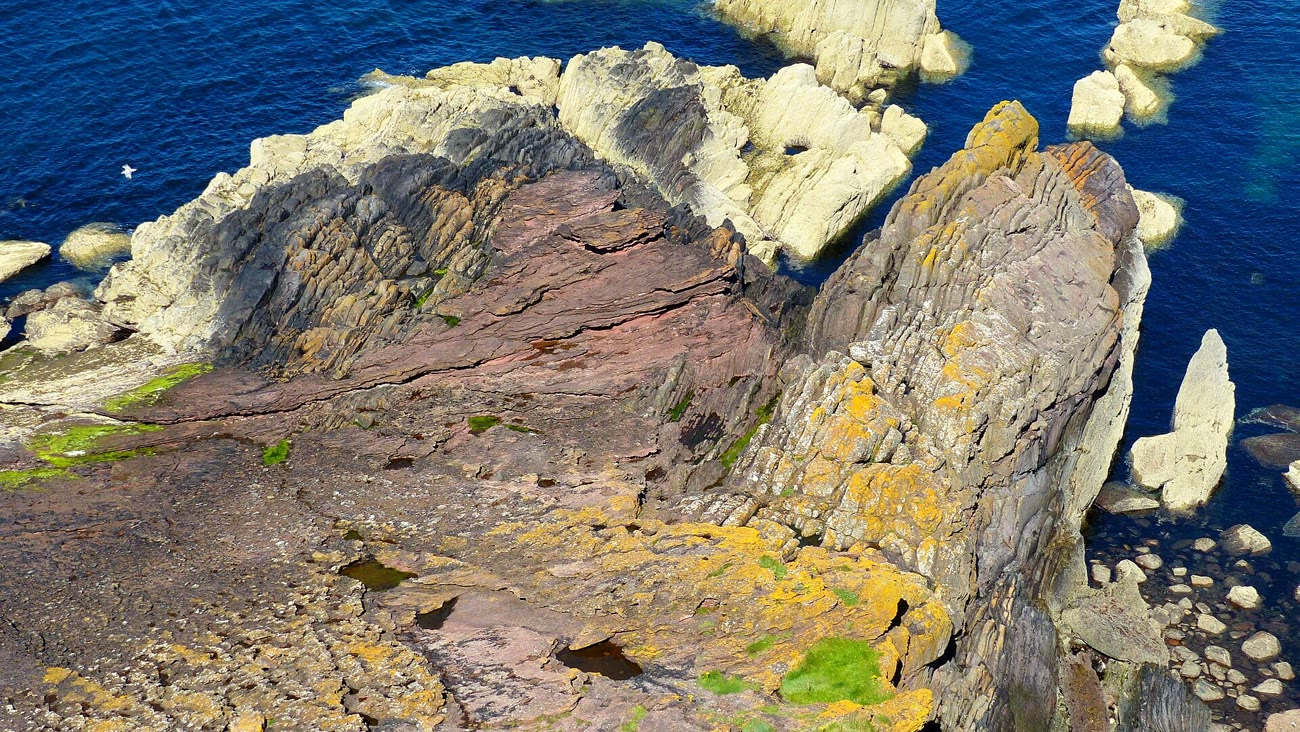
\includegraphics[width=0.7\linewidth]{images/book3/b1-siccar-point.jpg}

{\small \omterm{def:b1:cross-sections:unconformity}{عدم التوافق} عند سيكار بوينت لهاتون: طبقات رمادية سيلورية شبه شاقولية أسفل، وطبقات حمراء ديفونية مائلة برفق أعلى. الصورة: PawełS، بترخيص CC BY-SA 4.0 (Wikimedia Commons).}
% ledger: commons:siccar-point
\end{center}
\end{history}

\begin{inthefield}[جيولوجيا لنفق]
\begin{minipage}[t]{0.6\linewidth}\vspace{0pt}
قبل تصميم النفق، يبني الجيولوجيون الهندسيون مقاطع على طول خطه انطلاقًا من \omterm{def:b1:geological-maps:geological-map}{الخريطة الجيولوجية}، ومن الآبار التي تُحفر على فترات على امتداد المسار، ومن المسوحات الجيوفيزيائية. فيتنبأون بكل وحدة سيقطعها النفق، وبالصدوع التي سيعبرها، والمواضع التي قد يدخل فيها الماء. وأثناء الحفر يسجّل جيولوجيو المقاول الصخر المكشوف على الوجه عند كل تقدّم، ويقارنونه بالتنبؤ، ويحدّثون المقطع؛ وتُحفر آبار تجريبية أمام الآلة لتختبر الأرض قبل أن تصل إليها الآلة، وبخاصة قرب صدع متوقّع أو في حجر جيري قد يحوي تجاويف. وتُعدّ منطقة الصدع المكوّنة من صخر مسحوق خطرًا كلاسيكيًا، وأشدّ من ذلك حين يكون الصخر نفسه على الجانبين، ولا شيء في الوجه ينذر به.
\end{minipage}\hfill
\begin{minipage}[t]{0.37\linewidth}\vspace{0pt}
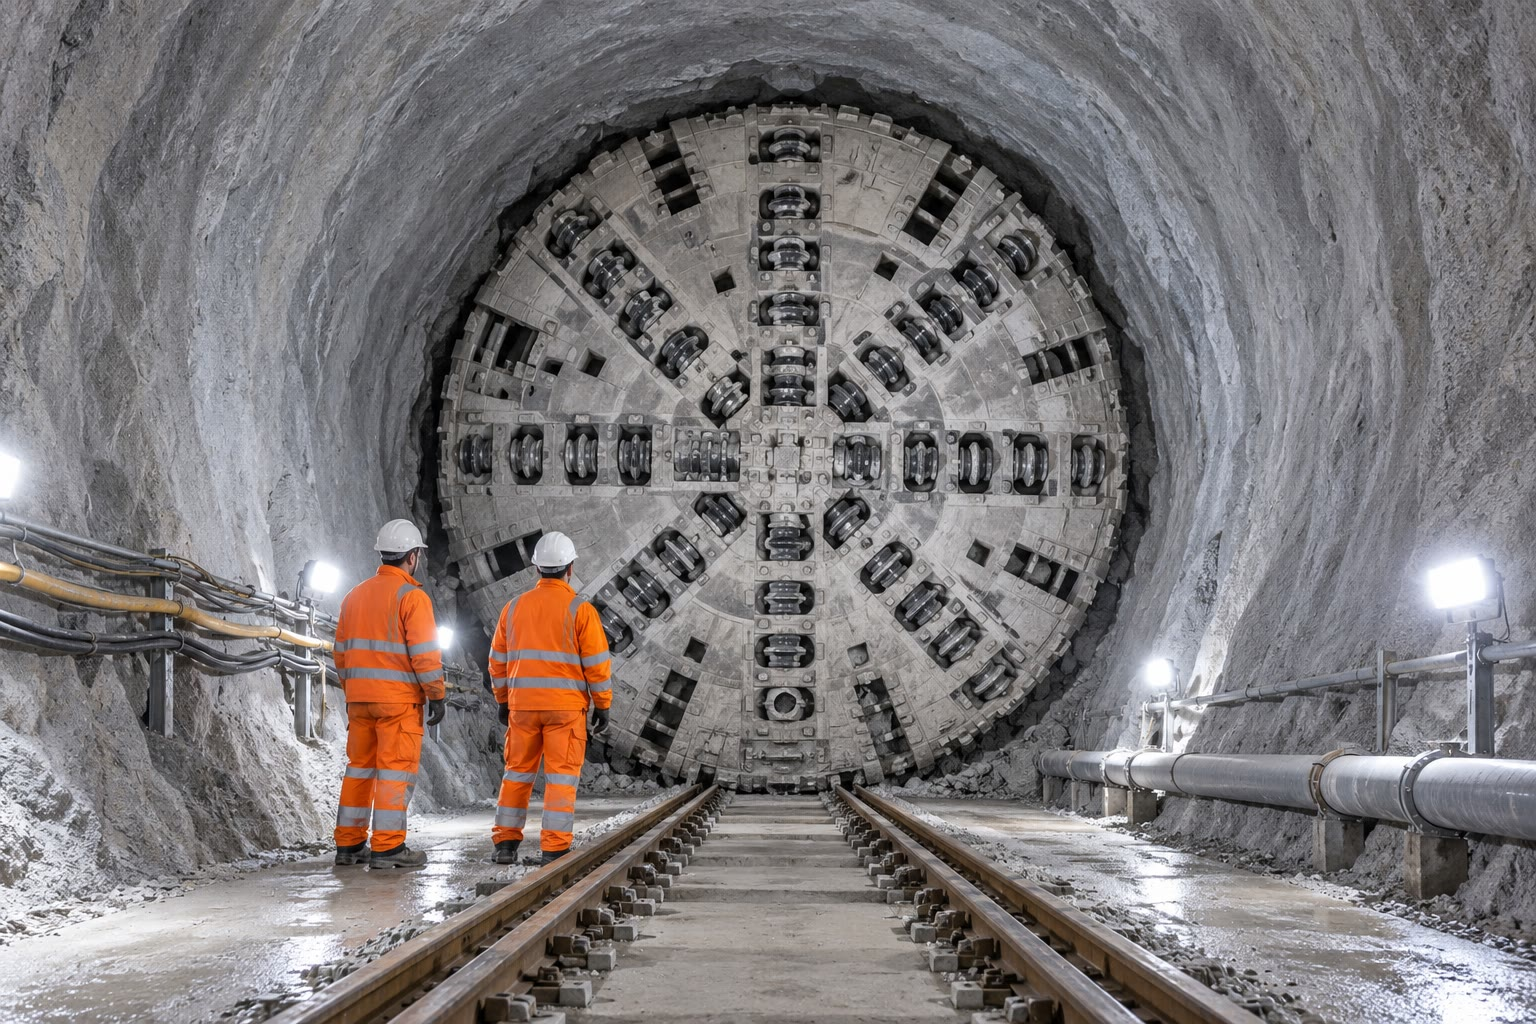
\includegraphics[width=\linewidth]{images/book3/ai/b1-tunnel-boring.jpg}
\end{minipage}
\end{inthefield}

\section{التمارين}

\begin{exercise}[$\star$]\label{exo:b1:cross-sections:1}
يُرسم مقطع من خريطة بمقياس 1:25\,000، ومقياسه الرأسي \qty{1}{cm} لكل \qty{100}{m}. ما مبالغته الرأسية؟
\end{exercise}

\begin{exercise}[$\star$]\label{exo:b1:cross-sections:2}
تنحدر طبقة بزاوية \ang{40} نحو \ang{090}. ما انحدارها الظاهري في مقطع شاقولي سمته \ang{060}؟ وفي مقطع سمته \ang{000}؟
\end{exercise}

\begin{exercise}[$\star$]\label{exo:b1:cross-sections:3}
يقطع بئر شاقولي \qty{120}{m} من الحجر الرملي تنحدر طبقاته بزاوية \ang{12.16}. ما \omterm{def:b1:cross-sections:thickness}{السمك الحقيقي} للحجر الرملي؟
\end{exercise}

\begin{exercise}[$\star$]\label{exo:b1:cross-sections:4}
يُرسم \omterm{def:b1:geological-maps:geological-map}{تماس} ينحدر بزاوية \ang{12} في مستوي مقطع بمبالغات رأسية قدرها 2 و3 و5. بأيّ زوايا يظهر؟
\end{exercise}

\begin{exercise}[$\star\star$]\label{exo:b1:cross-sections:5}
تنحدر طبقة بزاوية \ang{25}. ينكشف عرضها \qty{300}{m}، مقيسًا عموديًا على \omterm{def:b1:geological-maps:attitude}{الامتداد}. احسب سمكها الحقيقي (أ) على أرض أفقية؛ (ب) على أرض تنحدر بزاوية \ang{10} عكس \omterm{def:b1:geological-maps:attitude}{اتجاه الانحدار}، مع قياس العرض على طول الأرض؛ (ج) على أرض تنحدر بزاوية \ang{10} في الاتجاه نفسه الذي ينحدر فيه \omterm{def:b1:geological-maps:attitude}{الانحدار}.
\end{exercise}

\begin{exercise}[$\star\star$]\label{exo:b1:cross-sections:6}
تُظهر طبقة انحدارًا ظاهريًا قدره \ang{20} نحو الشمال في مقطع شمالي جنوبي، و\ang{30} نحو الشرق في مقطع شرقي غربي. أوجد اتجاه انحدارها وانحدارها الحقيقي.
\end{exercise}

\begin{exercise}[$\star\star$]\label{exo:b1:cross-sections:7}
ينحدر أساس الحجر الجيري على الجناح الشرقي بزاوية \ang{12.16}. ما التباعد الأفقي لكنتوراته البنيوية المرسومة كل \qty{100}{m}؟ تحقّق منه على \omterm{def:b1:cross-sections:structure-contour}{مخطط الكنتورات البنيوية}.
\end{exercise}

\begin{exercise}[$\star\star$]\label{exo:b1:cross-sections:8}
من جدول الآبار، احسب ارتفاع قاعدة الصخر الطيني في B1 وB3. وفوق B2 تآكل الصخر الطيني: فمن \omterm{def:b1:cross-sections:thickness}{السمك الشاقولي} للحجر الجيري، أوجد الارتفاع الذي ستكون عنده قاعدته هناك، \omterm{def:b1:cross-sections:apparent-dip}{والانحدار الظاهري} لذلك \omterm{def:b1:geological-maps:geological-map}{التماس} بين B1 وB2 في المقطع C--D. ماذا تخبرنا مقارنة B1 وB3 عن \omterm{def:b1:geological-maps:fold}{الطية}؟
\end{exercise}

\begin{exercise}[$\star\star$]\label{exo:b1:cross-sections:9}
ينحدر صدع عادي بزاوية \ang{50} نحو \ang{180}، وله \omterm{def:b1:cross-sections:throw}{إزاحة رأسية} قدرها \qty{150}{m}. احسب \omterm{def:b1:cross-sections:throw}{إزاحته الأفقية}. وفي مقطع شاقولي سمته \ang{150}، ما \omterm{def:b1:cross-sections:apparent-dip}{الانحدار الظاهري} للصدع، وما الفصل بين القطعين السطحيين لطبقة أفقية على طول المقطع؟
\end{exercise}

\begin{exercise}[$\star\star\star$]\label{exo:b1:cross-sections:10}
بالنسبة إلى طبقة تنحدر بزاوية \ang{40}، في أي اتجاهات للمقطع يكون \omterm{def:b1:cross-sections:apparent-dip}{الانحدار الظاهري} نصف \omterm{def:b1:geological-maps:attitude}{الانحدار} الحقيقي، أي \ang{20}؟ بيّن أن \omterm{def:b1:cross-sections:apparent-dip}{الانحدار الظاهري} يتغيّر قليلًا قرب \omterm{def:b1:geological-maps:attitude}{اتجاه الانحدار}، وبسرعة قرب \omterm{def:b1:geological-maps:attitude}{الامتداد}.
\end{exercise}

\begin{exercise}[$\star\star\star$]\label{exo:b1:cross-sections:11}
يقطع بئر الحجر الجيري على الجناح الشرقي (\omterm{def:b1:cross-sections:thickness}{السمك الحقيقي} \qty{176.0}{m}، \omterm{def:b1:geological-maps:attitude}{والانحدار} \ang{12.16} نحو \ang{080.7}). ما طول اللبّ الذي يستخرجه (أ) إذا كان شاقوليًا؛ (ب) إذا كان مائلًا بزاوية \ang{60} تحت الأفق نحو \ang{260.7}؛ (ج) مائلًا بزاوية \ang{60} نحو \ang{080.7}؟ (إرشاد: الطول هو $t/\cos\psi$، حيث $\psi$ الزاوية بين البئر والناظم على التطبّق.)
\end{exercise}

\begin{exercise}[$\star\star\star$]\label{exo:b1:cross-sections:12}
عند \omterm{def:b1:cross-sections:unconformity}{عدم التوافق الزاوي}، تنحدر الطبقات السفلى بزاوية \ang{70} نحو \ang{090}، وتنحدر الطبقات العليا بزاوية \ang{20} نحو \ang{270}، مع \omterm{def:b1:geological-maps:attitude}{الامتداد} نفسه. دوّر \omterm{def:b1:geological-maps:geological-map}{الانكشاف} كله حول \omterm{def:b1:geological-maps:attitude}{الامتداد} لتعود الطبقات العليا أفقية: ما كان انحدار الطبقات السفلى حين رُسبت العليا؟ اكتب تاريخ \omterm{def:b1:geological-maps:geological-map}{الانكشاف} بالترتيب.
\end{exercise}

\section{مسألة: نفق تحت تلال فاردن}

\begin{problem}[{مسألة نهاية الأسبوع --- أيّ الصخور سيقطعها النفق، وأين يلاقي الصدع، وكم من الحجر الجيري سيحفره}]
\label{pb:b1:cross-sections:1}
% numbers from figdata/bachelor-1/varden_sections.py (model region.py) and the scratch calculator
يمتد النفق شرقًا مباشرةً على الخط C--D ($y = \qty{6}{km}$) على الارتفاع الثابت \qty{200}{m}، من $x = \qty{1}{km}$ إلى $x =
\qty{9}{km}$. وارتفاع الأرض على طول C--D، كل كيلومتر ابتداءً من $x = 0$، هو:
\begin{center}
\small
\begin{tabular}{lccccccccccc}
\hline
$x$ \babelsublr{(km)} & \mbox{\textdir TLT 0} & \mbox{\textdir TLT 1} & \mbox{\textdir TLT 2} & \mbox{\textdir TLT 3} & \mbox{\textdir TLT 4} & \mbox{\textdir TLT 5} & \mbox{\textdir TLT 6} & \mbox{\textdir TLT 7} & \mbox{\textdir TLT 8} & \mbox{\textdir TLT 9} & \mbox{\textdir TLT 10} \\
$z$ \babelsublr{(m)} & \mbox{\textdir TLT 509} & \mbox{\textdir TLT 556} & \mbox{\textdir TLT 467} & \mbox{\textdir TLT 370} & \mbox{\textdir TLT 435} & \mbox{\textdir TLT 534} & \mbox{\textdir TLT 501} & \mbox{\textdir TLT 455} & \mbox{\textdir TLT 406} & \mbox{\textdir TLT 339} & \mbox{\textdir TLT 405} \\
\hline
\end{tabular}
\end{center}
استعمل جدول الآبار في الفصل، والمقطع C--D المرسوم بالمبالغة $e = 3$، \omterm{def:b1:geological-maps:attitude}{ووضعية} الجناح الشرقي (انحداره \ang{12.16} نحو \ang{080.7}؛ والجناح الغربي صورته المرآتية، ينحدر نحو \ang{279.3})، والصدع العادي، الذي ينحدر بزاوية \ang{60} نحو \ang{120}، وله \omterm{def:b1:cross-sections:throw}{إزاحة رأسية} قدرها \qty{200}{m}، ويمرّ بالنقطة $x = \qty{4.30}{km}$، $y = \qty{1.00}{km}$،
$z = \qty{250}{m}$.

\medskip
\noindent\textbf{الجزء الأول --- \omterm{def:b1:cross-sections:section}{المقطع الطبوغرافي} والوحدات.}
\begin{enumerate}
  \item ما أكبر سُمك وأصغره للصخر فوق النفق عند النقاط الكيلومترية بين $x = 1$ و$x = 9$؟
  \item على المقطع المطبوع، تقيس \qty{1}{km} من المسافة الأفقية \qty{1.4}{cm}، وتقيس \qty{1}{km} من الارتفاع \qty{4.2}{cm}. تحقّق من أن $e = 3$.
  \item من السجلّ B2، أوجد ارتفاع قاعدة الحجر الرملي على قمة \omterm{def:b1:geological-maps:fold}{الطية المحدبة}.
  \item في أيّ وحدة يقع النفق عند $x = \qty{3.5}{km}$؟
  \item احسب ارتفاع قاعدة الحجر الجيري في B1 وB3.
  \item من المقطع، اذكر بالترتيب الوحدات التي يعبرها النفق من $x = 1$ إلى $x = \qty{9}{km}$.
\end{enumerate}

\medskip
\noindent\textbf{الجزء الثاني --- الانحدارات في المقطع.}
\begin{enumerate}[resume]
  \item احسب \omterm{def:b1:cross-sections:apparent-dip}{الانحدار الظاهري} للجناح الشرقي في C--D من وضعيته.
  \item تحقّق منه من ارتفاعات قاعدة الحجر الجيري في B2 وB3.
  \item بأيّ زاوية يُرسم الجناح الشرقي في المقطع بالمبالغة $e = 3$؟
  \item احسب \omterm{def:b1:cross-sections:apparent-dip}{الانحدار الظاهري} للصدع في C--D.
  \item لماذا يكون \omterm{def:b1:cross-sections:apparent-dip}{الانحدار الظاهري} للجناحين في C--D قريبًا جدًا من انحدارهما الحقيقي، ولكن \omterm{def:b1:cross-sections:apparent-dip}{الانحدار الظاهري} للصدع أقلّ قربًا منه؟
\end{enumerate}

\medskip
\noindent\textbf{الجزء الثالث --- الصدع.}
\begin{enumerate}[resume]
  \item بيّن أنه على المستوي $y = \qty{6}{km}$ يقع الصدع عند
        \[ x = 4300 + \frac{2500 - (z - 250)\tan\ang{30}}{\sin\ang{120}}
           \quad\text{(بالأمتار)}. \]
  \item أين يلاقي النفق الصدع؟
  \item احسب \omterm{def:b1:cross-sections:throw}{الإزاحة الأفقية} للصدع، وفصل قطعتي \omterm{def:b1:geological-maps:geological-map}{تماس} على طول C--D.
  \item أيّ كتلة هبطت، وأيّ وحدة تقع على مستوى النفق في كل جانب من الصدع؟
  \item لماذا يكون الصدع خطرًا لا يستطيع طاقم الحفر أن يراه قادمًا من الصخر على الوجه؟ وكيف يحمي المهندسون أنفسهم منه؟
\end{enumerate}

\medskip
\noindent\textbf{الجزء الرابع --- الحجر الجيري.}
\begin{enumerate}[resume]
  \item ما \omterm{def:b1:cross-sections:thickness}{السمك الشاقولي} للحجر الجيري في B1؟
  \item ما سمكه الحقيقي؟
  \item بيّن أنه غرب الصدع على C--D تقع قاعدة الحجر الرملي عند
        \[ z_b = 160.16 - |x - 3500|\tan\ang{12.0} \quad\text{(بالأمتار)}. \]
  \item يكون النفق في الحجر الجيري حين تقع قاعدته تحت \qty{200}{m} وقمته فوقه. بيّن أن ذلك يحدث من أجل $377.1 < |x - 3500|
        < 1224.0$.
  \item أعطِ النقاط الأربع التي يدخل عندها النفق الحجر الجيري ويخرج منه.
  \item بيّن أن الطول المحفور على كل جناح هو $h/\tan\beta$، حيث $h$ \omterm{def:b1:cross-sections:thickness}{السمك الشاقولي} و$\beta$ \omterm{def:b1:cross-sections:apparent-dip}{الانحدار الظاهري}، ثم احسبه.
  \item ما مجموع طول الحجر الجيري الذي يحفره النفق؟
\end{enumerate}
\end{problem}
